\documentclass{beamer}
\usepackage{fontspec}
\usepackage{xeCJK}
\setCJKmainfont{Noto Sans CJK SC}
\newfontfamily\Libertine[Mapping=tex-text]{Linux Libertine O}
\usetheme{Madrid}
\usecolortheme{crane}

\usepackage{mygb4e}
\renewcommand{\eachwordtwo}{\Libertine}
\usepackage[e,f,j]{mtg2e}
\usepackage{xcolor}
\renewcommand{\mtcitestyle}[1]{\textcolor{teal}{\textit{#1}}}
\newcommand{\msa}{\mtciteform}
\newcommand{\cmn}{\mtciteform}
\usepackage{expex}
\newcommand{\txx}[1]{\textcolor{blue}{\textbf{#1}}}
\newcommand{\zz}{\txx}
\usepackage[normalem]{ulem}
\newcommand{\cll}[1]{\uline{#1}}
\newcommand{\ul}[1]{\uline{#1}}

\usepackage[round]{natbib}


\title[Grammar]{Grammatical Features\\ based largely on Goddard (2005) Chapter 4.}
\author[Francis Bond]{Francis Bond}
\date{2024}
\AtBeginSection[]
{
  \begin{frame}
    \frametitle{Outline}
    \tableofcontents[currentsection]
  \end{frame}
}
\begin{document}

  \frame{\titlepage}

  \begin{frame}
    \frametitle{Outline}
    \tableofcontents
\end{frame}

\section{Classifiers}


\begin{frame}{What Are Classifiers?}
\begin{itemize}
    \item Classifiers categorize nouns based on salient properties.
    \item Found in noun phrases (NPs) with modifiers like quantifiers.
    \item Essential for grammaticality when quantifiers (e.g., numerals) are present.
    \item Classifiers categorize by physical, social, or functional traits.
    \item Used with numerals, vague quantifiers like "some", or even alone.
\end{itemize}
\end{frame}

\begin{frame}{The Role of Classifiers in NPs}
\begin{itemize}
    \item Classifier slot required for quantifier NPs.
    \item Used with vague quantifiers like "many" and "some."
    \item Classifiers can appear with or without a noun.
    \item Classifier systems categorize referents based on properties like shape or function.
    \item In certain NPs, the classifier is mandatory for grammaticality.
\end{itemize}
\end{frame}

\begin{frame}{Classifier Phrases}
\begin{itemize}
    \item Classifier and quantifier form a grammatical sub-phrase.
    \item Quantifier and classifier appear adjacent to each other.
    \item Can sometimes occur alone without a noun.
    \item These classifier phrases are common across East and Southeast Asian languages.
    \item Example languages include Thai, Malaysian, and Mandarin.
\end{itemize}
\end{frame}





\begin{frame}{Examples: Thai and Malaysian}
\begin{itemize}
    \item Thai and Malaysian demonstrate similar classifier behaviors.
    \item Classifiers are used next to quantifiers.
    \item Classifier-quantifier pairs can occur without a noun in responses.
    \item Questions often require classifiers in these languages.
\end{itemize}
\ex
\begingl
\gla Mǎa kı̀i tua? //
\glb dog how.many CL:animal //
\glft ‘How many dogs?’ //
\endgl
\xe
\ex
\begingl
\gla (Mǎa) sǎam tua. //
\glb dog three CL:animal //
\glft ‘Three (dogs).’ //
\endgl
\xe
\end{frame}

\begin{frame}{Examples: Malaysian}
\begin{itemize}
    \item Similar behavior with quantifiers and classifiers in Malaysian.
    \item Classifiers appear adjacent to quantifiers.
    \item Noun can be omitted in responses.
\end{itemize}
\ex
\begingl
\gla Berapa ekor anjing? //
\glb how.many CL:animal dog //
\glft ‘How many dogs?’ //
\endgl
\xe
\ex
\begingl
\gla Tiga ekor (anjing). //
\glb three CL:animal dog //
\glft ‘Three (dogs).’ //
\endgl
\xe
\end{frame}


\begin{frame}{Sortal Classifiers}

\begin{itemize}
\item \zz{sortal} classifiers are the prototypical numeral classifiers
\item they pick out salient features of the noun they
  classify\\ 
  \zz{kinds}, that is, semantic classes\\
  \zz{shape} (or size) 
\item \zz{general} classifiers are used as follows:
  \begin{itemize}
  \item   for the residue of nouns\\
    \jpn[I saw a dream]{yume-o 1-\cll{tu} mita}
  \item   as a default when no particular feature is salient \\
    \jpn[I bought exactly one book]{hon-o ch\=odo  1-\cll{tu} katta}
  \item   for underspecified referents\\
    \jpn[I want one thingamajig]{nantoka-ga 1-\cll{tu} hoshii}
  \end{itemize}

\end{itemize}

\citep{Bond:Paik:2011}

\end{frame}


\begin{frame}{Measure (Mensural) vs. Sortal Classifier Constructions}
\begin{itemize}
    \item Measure constructions quantify "mass" substances (e.g., water, butter).
    \item Sortal constructions categorize countable items.
    \item Measure constructions refer to shape-based or container units.
    \item Sortal categorize objects based on properties like function or shape.
    \item Sortal systems apply broadly, while measure constructions are limited.
\end{itemize}
\end{frame}

\begin{frame}{Examples of Measure Constructions}
\begin{itemize}
    \item Measure constructions often use shape-based units.
    \item Examples: "two cups of water," "two grains of sand."
    \item Unit counter constructions group items (e.g., "two pairs of shoes").
    \item Measure constructions differ from classifiers structurally.
\end{itemize}
\ex
\begingl
\gla 二 杯 の 水 //
\glb ni hai no mizu //
\glc two CL.cup of water //
\glft two cups of water //
\endgl
\xe
\end{frame}

\begin{frame}{Unit Counter (Group) Constructions}
\begin{itemize}
    \item Used for collective or group items (e.g., "two pairs of shoes").
    \item Unit counters single out items from a larger set.
    \item Structurally similar to classifiers but serve different purposes.
    \item Examples include: "two pieces of furniture," "two bunches of bananas."
    \item Not so common in Japanese
    \item Very common in English and Thai
\end{itemize}
\end{frame}

\begin{frame}{Common Classifier Examples}
\begin{table}
\begin{tabular}{|l|l|}
\hline
\textbf{Language} & \textbf{Classifier} \\
\hline
Thai & \textit{tua} (animals) \\
Mandarin & \textit{gè} (general) \\
Vietnamese & \textit{cái} (general) \\
Malay & \textit{orang} (people) \\
\hline
\end{tabular}
\caption{Common Classifiers in Asian Languages}
\end{table}
\begin{itemize}
    \item Some classifiers are specialized, while others are general (used for many objects).
    \item General classifiers are used when object specifics are unknown.
\end{itemize}
\end{frame}

\begin{frame}{Repeater Constructions}
\begin{itemize}
    \item Nouns can act as their own classifier in repeater constructions.
    \item Common when no specific classifier exists.
    \item Often seen in languages like Thai and Lao.
    \item Repeater constructions fill the classifier slot with the noun itself.
\end{itemize}
\ex
\begingl
\gla Mii taw dòòk-maj cak taw? //
\glb there.is vase flower how.many vase //
\glft ‘How many vases are there?’ //
\endgl
\xe
\end{frame}

% \begin{frame}{General Classifiers}
% \begin{itemize}
%     \item General classifiers are used across many objects.
%     \item Example: Mandarin \textit{gè}, Cantonese \textit{go}, Vietnamese \textit{cái}.
%     \item Often replace specific classifiers in casual speech.
%     \item Used when the object’s nature is irrelevant or unknown.
% \end{itemize}
% \end{frame}

\begin{frame}{Specialized Classifiers}
\begin{itemize}
    \item Some languages, like Korean and Khmer, have specialized classifiers.
    \item These may be used for royalty, teachers, or monks.
    \item Classifiers categorize people by social status in some languages.
    \end{itemize}
\ex
\begingl
\gla 何 名 様 です か //
\glb nan mei sama desu ka //
\glc what CL.people.HON HON is Q //
\glft How many people? //
\endgl
\xe
\ex
\begingl
\gla 三 人 です //
\glb san nin desu //
\glc three CL.people is //
\glft Three //
\endgl
\xe
    
\end{frame}

\begin{frame}{Prototype and Extensions in Classifiers}
\begin{itemize}
    \item Classifiers often exhibit polysemy (multiple related meanings).
    \item A central, or "prototype," meaning extends to other related uses.
    \item Example: Thai \textit{tua} applies to animals but extends to furniture and clothing.
\end{itemize}
 \begin{center}
\noindent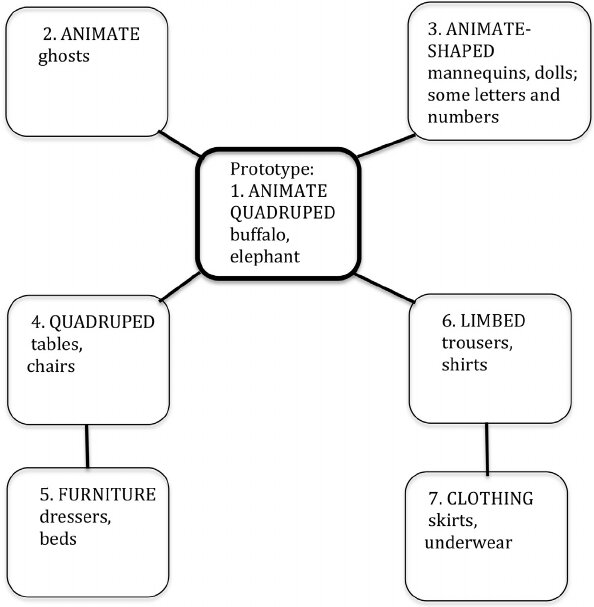
\includegraphics[height=0.6\textheight]{pics/Radial-category-structure-for-Thai-classifier-tua-Source-Adapted-from-Deepadung_W640.jpg}
 \end{center}
 %https://www.researchgate.net/publication/284094276_Slavic_aspectual_prefixes_and_numeral_classifiers_Two_kinds_of_lexico-grammatical_unitizers/figures
\end{frame}
\begin{frame}{Classifiers can indirectly count}
  \ex
  \begingl
  \gla 2-\cll{ts\=u}-no denshim\=eru (Japanese)//
  \glb 2-\cll{tong}-ui imayl (Korean) //
  \glc 2-CL.message-of email //
  \glft 2 \cll{pieces} of email//
  \endgl
  \xe
  \ex
  \begingl
  \gla 3-\cll{ts\=u}-no tegami (Japanese)//
  \glb 3-\cll{tong}-ui phyenci (Korean)//
  \glc 3-CL.message-of letter//
 \glft 3 letters           //%  \com{direct}
  \endgl
\xe
\ex
  \begingl
\gla  3-\cll{mai}-no tegami //
\glb  3-\cll{chang}-ui phyenci (Korean)//
\glc  3-CL.flat-of letter //
\glft \{a 3 \cll{page} letter/$^*$3 letters\}  //%\com{indirect}
  \endgl
  \xe

\end{frame}

\begin{frame}{Conclusion}
\begin{itemize}
    \item Classifiers categorize nouns based on physical, social, or functional traits.
    \item Found widely in East and Southeast Asian languages.
    \item Classifier systems vary from general to highly specialized.
    \item Classifiers are essential to noun phrase structure in these languages.
\end{itemize}
\end{frame}

\section{Aspect}

\begin{frame}{Aspect in East and Southeast Asian Languages}
\begin{itemize}
    \item Many East and Southeast Asian languages lack tense marking.
    \item Verbs are often marked for aspect instead of tense.
    \item Aspect marking can occur through suffixes, auxiliary verbs, or particles.
    \item Aspect focuses on the time structure of an event, not its time reference.
    \item Aspect can indicate whether an action is ongoing, completed, or habitual.
\end{itemize}
\end{frame}

\begin{frame}{What is Aspect?}
\begin{itemize}
    \item Aspect refers to the temporal structure of events.
    \item Different from tense, which indicates time reference (past, present, future).
    \item Example: English progressive aspect shows ongoing action (e.g. "is talking").
    \item Many East and Southeast Asian languages mark aspect using various strategies.
    \item Common aspect categories include perfective, imperfective, progressive, and habitual.
\end{itemize}
\end{frame}

\begin{frame}{Perfective vs. Imperfective Aspect}
\begin{itemize}
    \item Perfective aspect presents an event in its entirety.
    \item Imperfective aspect highlights the internal structure of an event.
    \item Imperfective can indicate ongoing (progressive), repeated (iterative), or habitual actions.
    \item Example: English progressive \eng{You are talking} is imperfective.
    \item Perfective focuses on completion, while imperfective focuses on duration or repetition.
\end{itemize}
\end{frame}

\begin{frame}{Types of Imperfective Aspect}
\begin{itemize}
    \item \txx{Progressive}: Ongoing action (e.g., "She is running").
    \item \txx{Iterative}: Repeated actions (e.g., "The light is flashing").
    \item \txx{Durative}: Actions that take time (e.g., "He was sitting").
    \item \txx{Habitual}: Regularly occurring actions (e.g., "She runs every morning").
    \item Imperfective aspects provide detailed temporal structure.
\end{itemize}
\end{frame}

\begin{frame}{Aspect in Sinitic Languages: Overview}
\begin{itemize}
    \item Aspect in Mandarin and Cantonese is marked using suffixes and particles.
    \item Different markers for perfective, progressive, continuous, and experiential aspects.
    \item Aspect marking is independent of tense (past, present, future).
    \end{itemize}
    \begin{table}
\begin{tabular}{lll}
\hline
\textbf{Aspect Type} & \textbf{Mandarin} & \textbf{Cantonese} \\
\hline
Perfective & le & jo \\
Progressive & zai & gan \\
Continuous & zhe & jyuh \\
Experiential & guo & gwo \\
\hline
\end{tabular}
\caption{Aspect markers in Mandarin and Cantonese}
\end{table}
\end{frame}

\begin{frame}{Perfective Aspect in Mandarin}
\begin{itemize}
    \item Perfective \cmn{le} indicates a completed action.
    \item Used in various contexts: past, future, or conditional events.
    \item Example: Conditional use of \cmn{le} in a future event.
\end{itemize}
\ex
\begingl
\gla Tā kāi-\ul{le} mén, nı̌ jiu jı̀n-qu. //
\glb 3sg open-perf door 2sg then enter-go //
\glft (Once) she opens the door, you go in. //
\endgl
\xe
\end{frame}

\begin{frame}{Perfective Aspect in Mandarin (continued)}
\begin{itemize}
    \item Perfective \cmn{le} can mark completion in different contexts.
    \item Can occur with specific objects, durations, or numbers of actions.
    \item Example: Perfective aspect with a stative verb (tall) and quantifier (a little).
\end{itemize}
\ex
\begingl
\gla Nı̌ gǎo-\ul{le} yı̄diǎn. //
\glb 2sg tall-perf a.little //
\glft You've got taller (a little). //
\endgl
\xe
\end{frame}

% \begin{frame}{Imperfective Aspects in Mandarin}
% \begin{itemize}
%     \item **Progressive zai**: Indicates ongoing action (e.g., "She is speaking").
%     \item **Continuous -zhe**: Marks continuous state (e.g., "The clouds are blocking").
%     \item **Experiential -guo**: Marks completed past experience, implying the action is over.
%     \item Usage of -guo contrasts with English perfect tense, implying the event is finished.
% \end{itemize}
% \end{frame}

\begin{frame}{Examples of Imperfective Aspects}
\ex
\begingl
\gla Wòhng sı́ujé góng-\ul{gán} dihnwá. //
\glb Wong miss talk-prog telephone //
\glft Miss Wong is talking on the phone.//
\endgl
\xe
\ex
\begingl
\gla Léih hái Hēunggóng jyuh-\ul{gwo} géi loih a? //
\glb you in Hong Kong live-exp how long prt //
\glft How long did you live in Hong Kong? //
\endgl
\xe
\end{frame}

\begin{frame}{Cantonese: Habitual Aspect}
\begin{itemize}
    \item Habitual aspect \cmn{hōi} marks regular or customary actions.
    \item Example: Habitual actions in present or past tense.
\end{itemize}
\ex
\begingl
\gla Kéuih jouh-\ul{hōi} jūngdı́m ge. //
\glb she work-hab part.time prt //
\glft ‘She normally works part-time.’ //
\endgl
\xe
\ex
\begingl
\gla Kéuih yı́hchı̀hn jā-\ul{hōi} Bēnsı́ ge. //
\glb she before drive-hab Benz prt //
\glft ‘She used to drive a Mercedes.’ //
\endgl
\xe
\end{frame}

\begin{frame}{Delimitative Aspect in Cantonese}
\begin{itemize}
    \item Delimitative \cmn{háh} indicates doing something "for a while."
    \item Often rendered as "have a V" in English.
    \item Example: "Have a look" or "have a walk."
\end{itemize}
\ex
\begingl
\gla Tái-\ul{háh}. //
\glb look-del //
\glft Have a look. //
\endgl
\xe
\ex
\begingl
\gla Yāusı̄k-\ul{háh}. //
\glb rest-del //
\glft Have a rest. //
\endgl
\xe
\end{frame}

\begin{frame}{Aspect Marking in Malaysian}
\begin{itemize}
    \item Aspect in Malaysian is marked by separate words before the verb.
    \item \msa{Sudah}  (perfective) and \msa{sedang} (progressive) are common markers.
    \item Perfective \msa{sudah} indicates completion, used for past or future events.
    \item \msa{Sedang} marks ongoing action, similar to the progressive in other languages.
\end{itemize}
\end{frame}

\begin{frame}{Examples of Malaysian Aspect}
\ex
\begingl
\gla Saya pun \ul{sudah} beritahu juga semalam. //
\glb I focus perf tell also yesterday //
\glft I already told (you) yesterday. //
\endgl
\xe
\ex
\begingl
\gla Bila saya masuk, dia \ul{sedang} membaca. //
\glb when I enter he prog read //
\glft When I came in, he was reading. //
\endgl
\xe
\end{frame}

\begin{frame}{Use in Singlish}
  \begin{itemize}
  \item This is carried over into Singapore Colloquial English (Singlish)
    \begin{itemize}
    \item \txx{habitual}: \eng{always}
    \item \txx{perfect}: \eng{already}
    \item \txx{progressive}: \eng{still}
    \end{itemize}
  \end{itemize}
  \ex   Eat \ul{already}?  ``Have you eaten''
  \xe
  \ex  Eat before class ``I ate before class''
  \xe
  \ex  He \ul{always} late one. ``He is habitually late''
  \xe
   \ex  Your phone \ul{still} spoil ah? ``Your phone is still broken?'' 
   \xe
\end{frame}


\begin{frame}{Conclusion on Aspect in East and Southeast Asian Languages}
\begin{itemize}
    \item Aspect marking is diverse across languages, with a variety of methods.
    \item Suffixes, particles, and separate words are used to indicate aspect.
    \item Common aspect categories include perfective, progressive, habitual, and delimitative.
    \item Each language has unique strategies for expressing temporal structure.
\end{itemize}
\end{frame}

\section{Serial Verbs}

\begin{frame}{Introduction to Serial Verb Constructions}
\begin{itemize}
    \item Serial verb constructions (SVCs) involve two or more verbs in a single clause.
    \item No conjunctions are used between the verbs.
    \item All verbs share the same grammatical subject.
    \item Common in East and Southeast Asian languages.
    \item Serial verb constructions serve various grammatical functions.
\end{itemize}
\end{frame}

\begin{frame}{Loose vs. Tight Serialization}
\begin{itemize}
    \item \txx{Loose serialization}: Verbs are loosely connected, depicting sequences of events.
    \item \txx{Tight serialization}: Verbs are tightly connected, representing a single event.
    \item In loose serialization, verbs may have independent arguments.
    \item Tight serialization often involves motion or posture verbs.
    \item Cultural factors can affect acceptability of tight serialization.
\end{itemize}
\end{frame}

\begin{frame}{Example of Loose Serialization (Lao)}
\begin{itemize}
    \item Loose serialization in Lao:
\end{itemize}
\ex
\begingl
\gla Dèèng paj$^3$ talaat$^5$ sùù$^4$ khùang$^1$ maa$^2$ hùan$^2$ lèèw$^4$. //
\glb Deng go market buy stuff come house perf //
\glft Deng went to the market, bought some stuff, (and) came home. //
\endgl
\xe
\begin{itemize}
    \item Verbs describe sequential actions.
    \item Perfective aspect marker applies to the entire sequence.
\end{itemize}
\end{frame}

\begin{frame}{Example of Tight Serialization (Thai)}
\begin{itemize}
    \item Tight serialization in Thai:
\end{itemize}
\ex
\begingl
\gla Dèk wı̂ng pay sı́i khanǒm. //
\glb child run go buy candy //
\glft The child ran (and) bought candy. //
\endgl
\xe
\begin{itemize}
    \item Verbs depict a single unitary event.
    \item Verbs share the same subject and object.
\end{itemize}
\end{frame}

\begin{frame}{Cultural Factors in Tight Serialization}
\begin{itemize}
    \item Cultural norms influence acceptability of verb combinations.
    \item Example: Playing musical instruments in Lao.
\end{itemize}
\ex
\begingl
\gla nang1 tii$^3$ lanaat$^4$. //
\glb sit beat lanaat //
\glft Play the lanaat sitting. //
\endgl
\xe
\ex
\begingl
\gla nòòn2 tii$^3$ lanaat$^4$. //
\glb lie beat lanaat //
\glft Play the lanaat lying down. //
\endgl
\xe
\begin{itemize}
    \item Playing the lanaat lying down is culturally unexpected.
    \item Context can make such constructions acceptable.
\end{itemize}
\end{frame}

\begin{frame}{Serial Verbs and Directional Verbs (Thai)}
\begin{itemize}
    \item Verbs like ‘go’ and ‘come’ often indicate direction in serial verb constructions.
    \item These directional verbs function similarly to adverbs.
    \item Example from Thai:
\end{itemize}
\ex
\begingl
\gla Khǎw klàp maa lÉEw. //
\glb 3sg return hither(come) perf //
\glft ‘She came back already.’ //
\endgl
\xe
\ex
\begingl
\gla Khǎw klàp pay lÉEw. //
\glb 3sg return away(go) perf //
\glft ‘She went back already.’ //
\endgl
\xe
\end{frame}

\begin{frame}{Three-Verb Serialization in Lao}
\begin{itemize}
    \item Serial verb constructions can include three verbs.
    \item First verb: manner of motion.
    \item Second verb: absolute direction (e.g., ‘up’, ‘down’).
    \item Third verb: direction relative to the speaker (e.g., ‘come’, ‘go’).
\end{itemize}
\ex
\begingl
\gla Laaw2 ñaang1 khùn5 maa2. //
\glb 3sg walk go.up come //
\glft ‘She walked up here.’ //
\endgl
\xe
\end{frame}

\begin{frame}{Verb-Prepositions in Serial Constructions}
\begin{itemize}
    \item Certain verbs take on grammatical functions similar to prepositions.
    \item Verbs like ‘give’, ‘use’, ‘go’ mark arguments such as beneficiaries or instruments.
    \item Example from Lao: haj5 ‘give’ functions as ‘for’.
\end{itemize}
\ex
\begingl
\gla Laaw2 nùng1 khaw5 haj5 khòòj5. //
\glb 3sg steam rice give(=for) 1sg //
\glft He steamed some rice for me. //
\endgl
\xe
\end{frame}

\begin{frame}{Comitative Use of Serial Verbs (Lao)}
\begin{itemize}
    \item Comitative ‘with’ often expressed using a serial verb construction.
    \item Example from Lao:
\end{itemize}
\ex
\begingl
\gla Khan2 haw2 juu1 nam2 mèè1-thaw5. //
\glb if we live accompany(=with) mother-old //
\glft If we live with your mother.’//
\endgl
\xe
\begin{itemize}
    \item Verb ‘accompany’ acts like a preposition meaning ‘with’.
\end{itemize}
\end{frame}

\begin{frame}{Serial Verbs in Vietnamese and Hmong}
\begin{itemize}
    \item Verb serialization marks locutionary topics in some languages.
    \item Example from Vietnamese: ‘arrive’ used for topics.
\end{itemize}
\ex
\begingl
\gla Chmng t\`\i nh@c d-Tn anh lu«n. //
\glb pl 1(excl.) recall arrive(=about) brother often //
\glft ‘We often speak about you.’ //
\endgl
\xe
\end{frame}
\begin{frame}{Serial Verbs form a cline in Japanese}
  
\begin{itemize}
\item Some serial verbs are completely lexicalized
  \begin{itemize}
  \item 取り締まる \jpn[manage (lit: take-squeeze)]{torishimaru}
  \end{itemize}
\item Some serial verbs are almost aspectual (like English particle verbs)
  \begin{itemize}
  \item 食べあげる \jpn[eat up (lit: eat rise)]{tabe-ageru}
  \item 歩きだす  \jpn[begin to walk/walk out (lit: walk leave)]{aruki-dasu}
  \end{itemize}
\item Some serial verbs are completely syntactic
  \begin{itemize}
  \item 食べおわる \jpn[finish eating (lit: eat finish)]{tabe-owaru}
  \item 歩きはじめる \jpn[start walking (lit: walk start)]{aruki-hajimeru}
  \end{itemize}
\item [!] Arguments can be transferred (in certani cases)
  \begin{itemize}
  \item 大阪を食べ歩く \jpn[stroll around Osaka eating (lit: Osaka walk eat)]{osaka-wo tabe-aruku}
  \item 寿司を食べ歩く \jpn[stroll around eating sushi (lit:  sushi walk eat)]{sushi-wo tabe-aruku}
  \end{itemize}
\end{itemize}
\citep{Hashimoto:Bond:2005}
\end{frame}


\begin{frame}{Summary of Serial Verb Constructions}
\begin{itemize}
    \item Serial verb constructions involve multiple verbs sharing a subject.
    \item They are common in East and Southeast Asian languages.
    \item They can express sequences, direction, beneficiary roles, and more.
    \item Loose serialization refers to sequences of events.
    \item Tight serialization depicts a single, unified event.
\end{itemize}
\end{frame}

\section{Subject and Topic}

\begin{frame}{What is a Subject?}
  \begin{itemize}
    \item NP preceding the verb holds a privileged position.
    \item English examples:
\ex
\ul{I} go
\xe
\ex
\ul{He} goes.
\xe
\ex
\ul{She} seems happy.
\xe
    \item Distinction of pronouns: *I* vs. *me*, *they* vs. *them*.
    \item Subject impacts verb agreement, e.g., -s in present tense.
    \item Subjects can be agents, patients, experiencers, etc.
  \end{itemize}
\end{frame}

\begin{frame}{Subject in Other Languages}
  \begin{itemize}
    \item Subject agreement in European languages.
    \item Case marking systems indicate subject (nominative).
    \item Verbs agree with subjects in person and number.
    \item Passive constructions highlight subjects:
    \ex
      Maxine was elected.
    \xe
    \item Traditional view: Subjects are universal in human languages.
  \end{itemize}
\end{frame}

\begin{frame}{Introduction to Topic}
  \begin{itemize}
    \item Topics define what the sentence is "about."
    \item Topics often overlap with subjects in English.
      \ex
      Cats eat mice (topic = cats).
      \xe
    \item In many Asian languages, topic and subject diverge.
    \item Topic prominence is perhaps more important than subject prominence in East Asian languages.
  \end{itemize}
\end{frame}

\begin{frame}{Topic Prominence: Thai}
  \begin{itemize}
    \item Flexible word order: OSV, SOV common in Thai.
    \item Example of OSV:
    \begin{example}
    \gll Pàakphanang khâaw raw kin ngâay. \\
         Pakphanang rice we eat simple \\
    \trans (In) Pakphanang, we ate simply.
    \end{example}
    \item Thai is typically SVO but informal sentences deviate.
    \item Widespread subject ellipsis in informal contexts.
    \item Pragmatic ordering of sentences.
  \end{itemize}
\end{frame}

\begin{frame}{Topic Prominence: Mandarin}
  \begin{itemize}
    \item Topics always appear sentence-initially.
    \item Example of topicalized object:
    \begin{example}
    \gll Zhāngsān wǒ yı̌jı̄ng jiàn-guo le. \\
         Zhangsan I already see-exp crs \\
    \trans Zhangsan, I've already seen (him).
    \end{example}
    \item Subject ellipsis possible when context is clear.
    \item Time and locative phrases often function as topics.
    \item Example: \eng{In Taipei, one can eat well.}
  \end{itemize}
\end{frame}

\begin{frame}{Topic vs. Subject in Mandarin}
  \begin{itemize}
    \item Flexible topic-comment structure.
    \item Double-subject construction in Mandarin.
    \item Example:
    \begin{example}
    \gll Xiàng bı́zi cháng. \\
         elephant nose long \\
    \trans ‘Elephants, (their) noses are long.’
    \end{example}
    \item Topic sets the frame for comment on the subject.
    \item The topic-comment structure is common and unmarked.
  \end{itemize}
\end{frame}

\begin{frame}{Topic and Subject in Japanese}
  \begin{itemize}
    \item \jpn{wa} marks topics, \jpn{ga} marks subjects.
    \item Example of \jpn{wa/ga} distinction:
      \ex
      \begingl
    \gla hi wa nobor-u. //
    \glb   sun top rise-pres //
    \glft The sun rises (general) //
    \endgl
    \xe
    \ex
          \begingl
    \gla hi ga nobor-u. //
     \glb     sun top rise-pres //
     \glft The sun is rising (specific) //
     \endgl
    \xe

    
    \item \jpn{wa} used in contrastive and generic statements.
    \item \jpn{ga} indicates a focus on the event as a whole.
    \item Adverbial topics: time/place phrases marked by \jpn{wa} (or unmarked)
  \end{itemize}
\end{frame}

\begin{frame}{Tagalog Trigger System}
  \begin{itemize}
    \item Tagalog has a flexible trigger system.
    \item Trigger denotes definiteness and is marked on verbs.
    \item Example of Actor Trigger (AT):
    \begin{example}
    \gll Mag-aalis ang bata ng laruan sa kahon. \\
         at-will.take.out trig child pat toy dir box \\
    \trans ‘The child will take a toy out of the box.’
    \end{example}
    \item Verb affixes indicate the role of the trigger NP.
    \item The system challenges traditional subject/topic definitions.
  \end{itemize}
\end{frame}

\begin{frame}{Actor vs. Undergoer in Acehnese}
  \begin{itemize}
    \item Acehnese verbs take person-marking prefixes or suffixes.
    \item Prefixes for actors, suffixes for undergoers.
    \item Example of Actor:
    \begin{example}
    \gll Geu-jak. \\
         3-go \\
    \trans ‘He/she goes.’
    \end{example}
    \item Example of Undergoer:
    \begin{example}
    \gll Lôn rhët-lôn. \\
         1sg fall-1sg \\
    \trans ‘I fall.’
    \end{example}
    \item Acehnese highlights actor/undergoer, not subject/object.
  \end{itemize}
\end{frame}

\begin{frame}{Summary: Subject and Topic}
  \begin{itemize}
    \item Subject prominence is common in European languages.
    \item Topic prominence is more evident in East Asian languages.
    \item Topic and subject do not always align.
    \item Languages like Tagalog and Acehnese challenge traditional subject concepts.
    \item Ongoing debates in linguistics about the universality of subjects.
  \end{itemize}
\end{frame}


\section{Sentence Final Particals (SFP)}

\begin{frame}{Illocutionary Particles Overview}
  \begin{itemize}
    \item Express speaker's immediate emotions, thoughts, desires.
    \item Common in Southeast Asian languages.
    \item Often sentence-final.
    \item Speech acts: requesting, questioning, persuading.
    \item Express emotional responses: surprise, doubt, hesitation.
  \end{itemize}
\end{frame}

\begin{frame}{Cantonese Sentence-Final Particles}
  \begin{itemize}
    \item Cantonese has over 30 basic particles.
    \item More than 100 particle combinations.
    \item Particles add subtle nuances to meaning.
    \item Function like English intonation but more explicit.
    \item Rich particle usage typical of Southeast Asian languages.
  \end{itemize}
\end{frame}

\begin{frame}{Examples of Cantonese Particles}
  \begin{table}[h]
    \centering
    \begin{tabular}{ll}
      \hline
      Particle & Meaning \\ \hline
      ā & lively statement, question \\ 
      áh & seeking confirmation \\ 
      ak & abrupt disagreement \\ 
      lā & requesting, seeking agreement \\ 
      lo & emphasizing current situation \\ 
      mē & expressing surprise \\
      wo & informative, noteworthy \\ 
      bo & exclamatory \\ 
      la & current relevance, advice \\ 
      ja & cheeky, intimate \\ 
    \end{tabular}
  \end{table}
\end{frame}

\begin{frame}{Examples of Cantonese Particles in Questions}
  \begin{itemize}
    \item \cmn{áh}: surprise or disapproval.
    \item \cmn{há}: presupposing agreement.
    \item \cmn{mē}: surprise, often in rhetorical questions.
  \end{itemize}
  \begin{example}
    \gll Léih gú gam yúhngyih áh? \\
         you guess so easy prt \\
    \trans ‘You think it's that easy, do you?’
  \end{example}
\end{frame}

\begin{frame}{Directive Particles}
  \begin{itemize}
    \item \cmn{la}: emphasizes a point of current relevance.
    \item \cmn{lo}: invites agreement or cooperation.
    \item Example sentences:
  \end{itemize}
  \begin{example}
    \gll Taai chóuh la, ngóh fan m̀h dóu. \\
         too noisy prt I sleep not prt \\
    \trans I can't sleep, it's too noisy.
  \end{example}
  \begin{example}
    \gll Gám jauh dāk lo. \\
         so then okay prt \\
    \trans ‘That'll be all right, won't it?’
  \end{example}
\end{frame}

\begin{frame}{Particles in Everyday Use}
  \begin{itemize}
    \item Particles appear very frequently in Cantonese speech.
    \item Average occurrence: every 1.5 seconds in conversation.
    \item Similar usage in Thai, Lao, and Vietnamese.
    \item Less frequent in formal settings or written texts.
    \item Frequency decreases in scientific or historical writing.
  \end{itemize}
\end{frame}

\begin{frame}{Mandarin Sentence-Final Particles}
  \begin{itemize}
    \item Mandarin has a smaller set of particles than Cantonese.
    \item Seven common particles in Mandarin.
    \item Example: \cmn{ma} (question), \cmn{ba} (suggestion), \cmn{ne} (emphasis).
    \item Particles are typical of informal, conversational settings.
    \item Estimated frequency: every six seconds in speech.
  \end{itemize}
\end{frame}

\begin{frame}{Examples of Mandarin Particles}
  \begin{example}
    \gll Nı̌ xı̌huan chı̄ ma? \\
         you like eat prt \\
    \trans ‘Do you like to eat?’
  \end{example}
  \begin{example}
    \gll Wǒmen qù ba. \\
         we go prt \\
    \trans ‘Let's go.’
  \end{example}
  \begin{example}
    \gll Tā ne? \\
         he prt \\
    \trans ‘What about him?’
  \end{example}
\end{frame}

\begin{frame}[allowframebreaks]{These are also common in Singlish}

  \ex You must go \ul{lah}. ``You must go, okay?"
\xe

\ex I already said \ul{lor}. ``I already told you, see?"
\xe

\ex  We're about to go already. Your friend  leh$^1$? \\ ``We're about to go already. What about your friend" (question)
\xe

\ex
Eh, don't like that leh$^3$. We need you here to play mahjong. \\ ``Don't be like that. We need you here to play mahjong.'' (persuasive)
\xe

\ex This one easy \ul{mah}. ``This one is easy, you know?"
\xe

\ex You sure can do it \ul{meh}? ``Are you really sure you can do it?"
\xe

\ex Don't blame me \ul{what}. ``It's not my fault, you know?"
\xe

\ex She always like that \ul{one}. ``She's always like that, you know?"
\xe

\citep{chow-etal-2024-word}
\end{frame}

\begin{frame}{Conclusion: Importance of Particles}
  \begin{itemize}
    \item Particles convey subtle shades of meaning in speech.
    \item Express emotions, intentions, and social cues.
    \item Different languages utilize particles with varying frequencies.
    \item Illocutionary particles are an areal feature of Southeast Asia.
    \item Essential in mastering conversational fluency in these languages.
  \end{itemize}
\end{frame}

\begin{frame}{Conclusions}
  \begin{itemize}
  \item SEA languages have many features not found in Indo-European languages
  \item They package up meaning in different ways
  \end{itemize}
\end{frame}

% \section{Some of my work}

% \begin{frame}{My research}
%   \begin{itemize}
%   \item Classifiers
%     \begin{itemize}
%     \item 
%     \end{itemize}
%   \item Tense
%   \item Serial Verbs
%   \item Sentence Final Particles
%   \end{itemize}
% \end{frame}

\begin{frame}[allowframebreaks]
        \frametitle{References}
        \bibliographystyle{aclnat}
        \bibliography{abb,mtg,ling,nlp}
\end{frame}


\end{document}
